\documentclass[11pt,a4paper]{article}
\usepackage[utf8]{inputenc}
\usepackage[T1]{fontenc}
\usepackage{lmodern}
\usepackage[portuguese]{babel}
\usepackage[a4paper,margin=2.4cm]{geometry}
\usepackage{xcolor}
\usepackage{graphicx}
\usepackage{titlesec}
\usepackage{enumitem}
\usepackage{listings}
\usepackage{tcolorbox}
\usepackage{booktabs}
\usepackage{amsmath}
\usepackage{amssymb}
\usepackage{fancyhdr}
\usepackage{hyperref}
\tcbuselibrary{skins,breakable,listings}

\definecolor{BgCream}{HTML}{FAF8F5}
\definecolor{TextEspresso}{HTML}{4A4238}
\definecolor{NudeTaupe}{HTML}{BFAFA6}
\definecolor{SoftBlush}{HTML}{D9C5B2}
\definecolor{SageMuted}{HTML}{7E8F7C}
\definecolor{ClayWarn}{HTML}{B5795C}

\hypersetup{colorlinks=true, linkcolor=TextEspresso, urlcolor=TextEspresso}

\titleformat{\section}{\color{TextEspresso}\Large\bfseries}{\thesection}{0.6em}{}[{\color{NudeTaupe}\titlerule[0.8pt]}]
\titleformat{\subsection}{\color{TextEspresso}\large\bfseries}{\thesubsection}{0.6em}{}
\titlespacing*{\section}{0pt}{1.4\baselineskip}{0.7\baselineskip}
\titlespacing*{\subsection}{0pt}{1.1\baselineskip}{0.5\baselineskip}

\lstset{
  basicstyle=\ttfamily\small,
  breaklines=true,
  columns=fullflexible,
  showstringspaces=false,
  frame=none,
  aboveskip=0pt, belowskip=0pt
}

\pagestyle{fancy}
\fancyhf{}
\renewcommand{\headrulewidth}{0pt}
\fancyfoot[C]{\color{NudeTaupe}\small\thepage}

% ---- Caixa: comandos a executar ----
\newtcblisting{terminal}{
  listing only, breakable,
  colback=BgCream, colframe=NudeTaupe,
  boxrule=0.5pt, arc=2pt, left=6pt, right=6pt, top=5pt, bottom=5pt,
  listing options={basicstyle=\ttfamily\small, breaklines=true, columns=fullflexible}
}

% ---- Caixa: saida esperada ----
\newtcblisting{saida}{
  listing only, breakable,
  colback=white, colframe=SoftBlush,
  boxrule=0.5pt, arc=2pt, left=6pt, right=6pt, top=5pt, bottom=5pt,
  title={\small\bfseries\color{TextEspresso}Saída esperada},
  coltitle=TextEspresso, colbacktitle=SoftBlush!45,
  fonttitle=\small\bfseries,
  listing options={basicstyle=\ttfamily\footnotesize, breaklines=true, columns=fullflexible}
}

% ---- Caixa: ponto de verificacao ----
\newtcolorbox{verificar}{
  breakable, colback=SageMuted!8, colframe=SageMuted,
  boxrule=0.6pt, arc=2pt, left=7pt, right=7pt, top=6pt, bottom=6pt,
  title={\small\bfseries Confirme antes de avançar},
  coltitle=white, colbacktitle=SageMuted, fonttitle=\small\bfseries
}

% ---- Caixa: aviso ----
\newtcolorbox{atencao}{
  breakable, colback=ClayWarn!8, colframe=ClayWarn,
  boxrule=0.6pt, arc=2pt, left=7pt, right=7pt, top=6pt, bottom=6pt,
  title={\small\bfseries Atenção},
  coltitle=white, colbacktitle=ClayWarn, fonttitle=\small\bfseries
}

% ---- Caixa: nota/contexto ----
\newtcolorbox{nota}{
  breakable, colback=NudeTaupe!10, colframe=NudeTaupe,
  boxrule=0.5pt, arc=2pt, left=7pt, right=7pt, top=6pt, bottom=6pt
}

% ---- Cabecalho do manual ----
\newcommand{\manualtitle}[3]{%
  \thispagestyle{empty}
  \begin{center}
  {\color{NudeTaupe}\rule{\textwidth}{0.5pt}}\\[0.5cm]
  {\LARGE\bfseries\color{TextEspresso} Manual Técnico #1}\\[0.35cm]
  {\large\color{TextEspresso} #2}\\[0.3cm]
  {\normalsize\color{NudeTaupe} Infraestruturas de Computação na Nuvem \quad|\quad #3}\\[0.4cm]
  {\color{NudeTaupe}\rule{\textwidth}{0.5pt}}
  \end{center}
  \vspace{0.4cm}
}

% ---- Entrada de troubleshooting ----
\newcommand{\problema}[1]{\vspace{0.35cm}\noindent{\bfseries\color{TextEspresso}#1}\par\nopagebreak\vspace{0.1cm}}

\setlist[itemize]{itemsep=0.22cm, topsep=0.2cm}
\setlist[enumerate]{itemsep=0.22cm, topsep=0.2cm}

\begin{document}
\manualtitle{09}{Mensageria e Desacoplamento com RabbitMQ}{Aula 09}

\section*{Como usar este manual}

O objetivo central desta aula cabe numa frase: \textbf{ver o produtor continuar a funcionar quando o consumidor desaparece}. Tudo o resto é preparação para chegar a esse momento.

\begin{nota}
\textbf{Duas vias possíveis.} Este manual segue a via principal, com o cluster Kubernetes. Se o cluster não estiver disponível, a secção «Via alternativa com Docker» no fim permite fazer as partes essenciais dentro da VM \texttt{icn-lab}.
\end{nota}

\section*{Antes de começar}

\begin{itemize}
  \item[$\square$] Cluster Kubernetes com dois nós \texttt{Ready} (ou VM com Docker, para a via alternativa)
  \item[$\square$] \emph{Taint} do control plane removido -- necessário para o exercício de anti-affinity da Parte 6:
\begin{terminal}
$ kubectl taint nodes --all node-role.kubernetes.io/control-plane- 2>/dev/null
\end{terminal}
  \item[$\square$] Dois ou três terminais SSH abertos
  \item[$\square$] Acesso ao Proxmox para o teste final
\end{itemize}

\section{Implantar o RabbitMQ}

\subsection{Aplicar o manifesto}

\begin{terminal}
$ nano rabbitmq.yaml
\end{terminal}

Copie o conteúdo do Guião 09.

\begin{terminal}
$ kubectl apply -f rabbitmq.yaml
$ kubectl get pods -l app=rabbitmq --watch
\end{terminal}

\begin{atencao}
O arranque demora \textbf{30 a 60 segundos}. Espere pelo estado \texttt{Running} com \texttt{1/1} na coluna \texttt{READY}. Se avançar antes disso, as ligações vão falhar. Interrompa o \texttt{--watch} com \texttt{Ctrl+C} quando estiver pronto.
\end{atencao}

\subsection{Aceder à interface de gestão}

Abra no browser:
\begin{terminal}
http://<IP-de-um-no>:31672
\end{terminal}

Credenciais: as que definiu no Secret (\texttt{aluno} / \texttt{aulaicn2026}).

\begin{verificar}
Entrou na interface e vê os separadores \emph{Overview}, \emph{Connections}, \emph{Exchanges} e \emph{Queues}. Vai usá-los ao longo da aula para ver o que se passa por dentro.
\end{verificar}

\subsection{Confirmar o DNS interno}

\begin{terminal}
$ kubectl run dns-teste --rm -it --image=busybox:1.36 --restart=Never -- \
    nslookup rabbitmq
\end{terminal}

\begin{saida}
Name:      rabbitmq
Address 1: 10.106.55.12 rabbitmq.default.svc.cluster.local
\end{saida}

Os Pods poderão alcançar o broker pelo nome \texttt{rabbitmq}, sem saber o IP.

\section{Work queue}

\subsection{Preparar os scripts}

\begin{terminal}
$ nano worker.py
\end{terminal}

Copie o \texttt{worker.py} do Guião 09. Dois detalhes que valem atenção:

\begin{itemize}
  \item \texttt{basic\_qos(prefetch\_count=1)} -- cada worker só recebe uma tarefa de cada vez, o que distribui o trabalho de forma justa.
  \item \texttt{basic\_ack} no fim do \texttt{callback} -- confirma o processamento. Sem esta confirmação, o broker volta a entregar a mensagem a outro worker.
\end{itemize}

\subsection{Injetar o código no cluster}

\begin{terminal}
$ kubectl create configmap worker-code --from-file=worker.py
$ kubectl get configmap worker-code
\end{terminal}

\begin{nota}
Usamos um ConfigMap para evitar construir e distribuir uma imagem própria. Em produção construir-se-ia uma imagem; aqui, para uma aula, isto é mais rápido.
\end{nota}

\subsection{Implantar os workers}

\begin{terminal}
$ nano worker.yaml
$ kubectl apply -f worker.yaml
$ kubectl get pods -l app=worker
\end{terminal}

\begin{atencao}
Cada Pod faz \texttt{pip install pika} ao arrancar, o que demora e exige acesso à Internet a partir dos nós. Espere que fiquem \texttt{Running}. Se ficarem em \texttt{Error} ou \texttt{CrashLoopBackOff}, veja os logs.
\end{atencao}

\subsection{Acompanhar os logs}

\textbf{Terminal 1:}
\begin{terminal}
$ kubectl logs -f -l app=worker --prefix --max-log-requests=10
\end{terminal}

\begin{saida}
[pod/worker-6c9f8d4b7-x2kp9/worker] [worker-6c9f8d4b7-x2kp9] A espera de tarefas.
[pod/worker-6c9f8d4b7-mz4tq/worker] [worker-6c9f8d4b7-mz4tq] A espera de tarefas.
\end{saida}

\subsection{Enviar tarefas}

A forma mais simples é pela interface web:

\begin{enumerate}
  \item Separador \textbf{Queues} $\rightarrow$ clique em \texttt{tarefas}
  \item Secção \textbf{Publish message}
  \item Em \emph{Payload}, escreva \texttt{tarefa 1}
  \item \textbf{Publish message}
  \item Repita com \texttt{tarefa 2}, \texttt{tarefa 3}, \texttt{tarefa 4}\ldots
\end{enumerate}

\begin{verificar}
No Terminal 1, as tarefas aparecem distribuídas por workers \emph{diferentes}. Cada tarefa é processada por \textbf{um} worker apenas. Registe a distribuição.
\end{verificar}

\subsection{Escalar os consumidores}

\begin{terminal}
$ kubectl scale deployment worker --replicas=4
$ kubectl get pods -l app=worker
\end{terminal}

Envie mais tarefas seguidas e compare o tempo total de processamento. Cada tarefa demora 2 segundos (\texttt{time.sleep(2)}): com 2 workers, 8 tarefas levam cerca de 8 segundos; com 4 workers, cerca de 4.

\section{Publish/subscribe}

Adapte o \texttt{worker.yaml} para os subscribers (mude o nome do Deployment, o ConfigMap e o script executado), usando o \texttt{subscribe\_event.py} do guião.

Publique um evento pela interface web, agora no exchange \texttt{eventos} (separador \textbf{Exchanges}).

\begin{verificar}
\textbf{Todos} os subscribers receberam a \emph{mesma} mensagem. Compare com a work queue, onde cada mensagem foi para \emph{um} consumidor só. A diferença está no tipo de exchange: \texttt{fanout} difunde, a fila directa distribui.
\end{verificar}

No separador \textbf{Queues} confirme que cada subscriber tem a sua própria fila temporária ligada ao exchange.

\section{O exercício central: desacoplamento}

\begin{center}
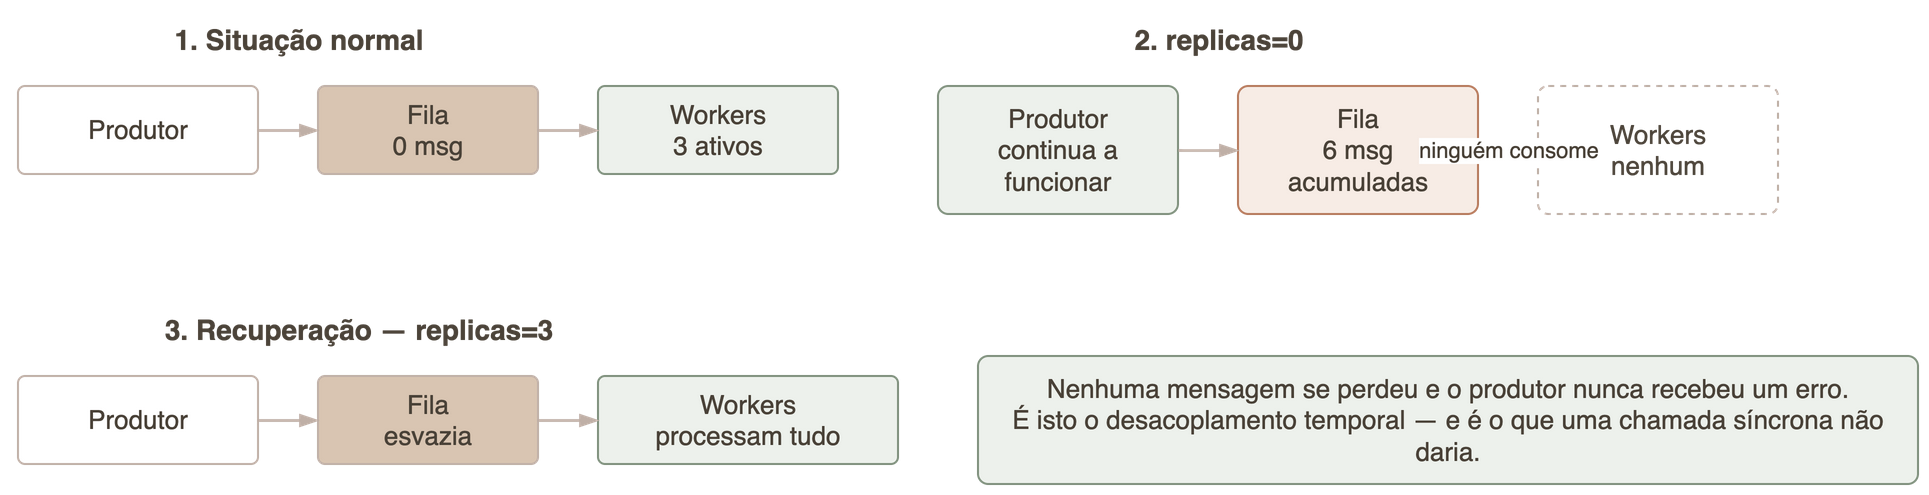
\includegraphics[width=\linewidth]{../Diagramas/m09-desacoplamento.png}\\[0.15cm]
{\small\color{NudeTaupe} O produtor nunca falha, mesmo sem nenhum consumidor ativo.}
\end{center}


\subsection{Desligar todos os consumidores}

\begin{terminal}
$ kubectl scale deployment worker --replicas=0
$ kubectl get pods -l app=worker
\end{terminal}

\begin{saida}
No resources found in default namespace.
\end{saida}

\subsection{Continuar a produzir}

Publique 5 ou 6 mensagens pela interface web, exatamente como antes.

\begin{verificar}
\textbf{O produtor funcionou normalmente.} Nenhum erro, nenhuma exceção, nenhuma espera -- apesar de não existir um único consumidor. É isto o desacoplamento temporal.
\end{verificar}

\subsection{Ver as mensagens acumuladas}

Na interface web, separador \textbf{Queues}, a coluna \emph{Ready} da fila \texttt{tarefas} mostra as mensagens à espera. Ou por linha de comandos:

\begin{terminal}
$ kubectl exec deployment/rabbitmq -- rabbitmqctl list_queues name messages
\end{terminal}

\begin{saida}
Listing queues ...
name       messages
tarefas    6
\end{saida}

Registe o número: \underline{\hspace{1.5cm}}

\subsection{Recuperar}

\begin{terminal}
$ kubectl scale deployment worker --replicas=3
$ kubectl logs -f -l app=worker --prefix --max-log-requests=10
\end{terminal}

\begin{verificar}
Os workers arrancaram e processaram \textbf{todas} as mensagens acumuladas, sem perda. O sistema recuperou sozinho de uma indisponibilidade total do lado consumidor.
\end{verificar}

\begin{nota}
Pense no que aconteceria numa chamada síncrona (REST direto): o produtor teria recebido erro de ligação em cada tentativa, e o trabalho ter-se-ia perdido — a menos que implementasse ele próprio filas, retries e persistência. A fila resolve isso de origem.
\end{nota}

\section{Durabilidade}

\begin{terminal}
$ kubectl scale deployment worker --replicas=0
\end{terminal}

Publique 3 mensagens. Depois reinicie o broker:

\begin{terminal}
$ kubectl rollout restart deployment rabbitmq
$ kubectl get pods -l app=rabbitmq --watch
\end{terminal}

Quando voltar a \texttt{Running}, verifique:

\begin{terminal}
$ kubectl exec deployment/rabbitmq -- rabbitmqctl list_queues name messages
\end{terminal}

\begin{atencao}
\textbf{As mensagens desapareceram} -- e isso é esperado. Este Deployment não tem armazenamento persistente: quando o Pod é recriado, começa de zero. As mensagens estavam marcadas como duráveis, mas a durabilidade escreve em disco, e o disco deste Pod é efémero.

Para as preservar seria preciso um \textbf{StatefulSet} com um \textbf{PersistentVolume}. Esta é a resposta a uma das questões de verificação.
\end{atencao}

\section{Redundância entre nós}

\subsection{Ver a distribuição}

\begin{terminal}
$ kubectl scale deployment worker --replicas=4
$ kubectl get pods -l app=worker -o wide
\end{terminal}

\subsection{Forçar distribuição por nós diferentes}

Acrescente o bloco \texttt{affinity} do Guião 09 ao \texttt{worker.yaml} e reaplique:

\begin{terminal}
$ kubectl apply -f worker.yaml
$ kubectl get pods -l app=worker -o wide
\end{terminal}

\begin{verificar}
Os Pods estão agora repartidos pelos dois nós, em vez de concentrados num só. Se um nó cair, sobrevivem os do outro.
\end{verificar}

\subsection{Testar a falha de nó}

\textbf{Na shell do node Proxmox:}
\begin{terminal}
$ qm stop <vmid-w1>
\end{terminal}

Publique mais mensagens e confirme que continuam a ser processadas pelos workers do nó sobrevivente.

\begin{terminal}
$ qm start <vmid-w1>
\end{terminal}

\section{Limpeza}

\begin{terminal}
$ kubectl delete -f worker.yaml
$ kubectl delete configmap worker-code
$ kubectl delete -f rabbitmq.yaml
$ kubectl get all
\end{terminal}

\section{Via alternativa com Docker}

Se o cluster não estiver disponível, na VM \texttt{icn-lab}:

\begin{terminal}
$ docker run -d --name rabbitmq \
    -p 5672:5672 -p 15672:15672 \
    -e RABBITMQ_DEFAULT_USER=aluno \
    -e RABBITMQ_DEFAULT_PASS=aulaicn2026 \
    rabbitmq:3-management
$ docker ps
\end{terminal}

Interface em \texttt{http://<IP-da-VM>:15672}. Instale o cliente e corra os scripts localmente:

\begin{terminal}
$ sudo apt install -y python3-pip
$ pip3 install pika
$ export RABBIT_HOST=localhost
$ python3 worker.py        # num terminal
$ python3 send_task.py "tarefa 1"   # noutro
\end{terminal}

O exercício central (secção 4) funciona igual: pare os workers com \texttt{Ctrl+C}, continue a enviar, e observe a fila a crescer.

\section{Problemas frequentes}

\problema{Os Pods do worker ficam em \texttt{CrashLoopBackOff}}
Veja a causa:
\begin{terminal}
$ kubectl logs -l app=worker --tail=30
\end{terminal}
As causas mais frequentes: o \texttt{pip install} falhou (sem Internet nos nós), ou o broker ainda não estava pronto quando o worker tentou ligar-se. No segundo caso, os Pods recuperam sozinhos ao fim de algumas tentativas.

\problema{\texttt{pika.exceptions.AMQPConnectionError}}
O broker não está acessível. Confirme:
\begin{terminal}
$ kubectl get pods -l app=rabbitmq
$ kubectl get svc rabbitmq
\end{terminal}
Confirme também que a variável \texttt{RABBIT\_HOST} está definida como \texttt{rabbitmq}.

\problema{\texttt{ACCESS\_REFUSED - Login was refused}}
Utilizador ou password errados. Têm de coincidir com o Secret. Verifique o que o broker tem:
\begin{terminal}
$ kubectl exec deployment/rabbitmq -- rabbitmqctl list_users
\end{terminal}

\problema{A interface web não abre em \texttt{:31672}}
Confirme que o Service tem a NodePort correta e experimente o IP do outro nó:
\begin{terminal}
$ kubectl get svc rabbitmq
\end{terminal}

\problema{As tarefas vão todas para o mesmo worker}
Falta o \texttt{basic\_qos(prefetch\_count=1)}, ou as tarefas foram enviadas antes de o segundo worker estar pronto. Confirme que ambos aparecem no separador \emph{Connections} da interface web.

\problema{\texttt{kubectl logs -l app=worker} só mostra um Pod}
Acrescente \texttt{--max-log-requests=10} e \texttt{--prefix}, para ver todos e saber qual é qual.

\problema{As mensagens ficam presas em \texttt{Unacked}}
Um worker recebeu a mensagem mas morreu antes do ACK. O broker volta a entregá-la quando a ligação cai. Se ficarem presas, reinicie os workers.

\section{Referência rápida}

\begin{center}
\begin{tabular}{@{}ll@{}}
\toprule
\textbf{Comando} & \textbf{Para que serve} \\
\midrule
\texttt{kubectl create configmap N -{}-from-file=f} & Injetar ficheiro no cluster \\
\texttt{kubectl logs -f -l app=X -{}-prefix} & Seguir logs de vários Pods \\
\texttt{kubectl scale deploy X -{}-replicas=0} & Desligar todos os consumidores \\
\texttt{kubectl rollout restart deploy X} & Recriar os Pods \\
\texttt{kubectl exec deploy/rabbitmq -- CMD} & Executar comando no broker \\
\midrule
\texttt{rabbitmqctl list\_queues name messages} & Mensagens por fila \\
\texttt{rabbitmqctl list\_users} & Utilizadores definidos \\
\texttt{rabbitmqctl list\_connections} & Ligações ativas \\
\bottomrule
\end{tabular}
\end{center}

\section{Checklist final}

\begin{itemize}
  \item[$\square$] O RabbitMQ está \texttt{Running} e acedo à interface de gestão
  \item[$\square$] Confirmei a resolução do nome \texttt{rabbitmq} por DNS interno
  \item[$\square$] Os workers arrancaram e vejo os logs de todos
  \item[$\square$] Registei a distribuição de tarefas pelos workers (work queue)
  \item[$\square$] Testei o publish/subscribe e confirmei que todos recebem a mesma mensagem
  \item[$\square$] \textbf{Reduzi os workers a zero e continuei a publicar sem erros}
  \item[$\square$] Registei o número de mensagens acumuladas na fila
  \item[$\square$] Voltei a escalar e as mensagens foram todas processadas
  \item[$\square$] Testei a durabilidade e sei explicar por que as mensagens se perderam
  \item[$\square$] Apliquei anti-affinity e confirmei a distribuição pelos nós
  \item[$\square$] Testei a falha de um nó com o sistema em funcionamento
  \item[$\square$] Limpei os recursos criados
\end{itemize}

\end{document}
